\chapter{Anden Iteration}
I dette afsnit beskrives 2. iteration af design- og implementeringsfasen. Den indebærer design og vikling af transformator samt valg af resterende komponenter i kredsløbet. Yderligere realiseres og testes hele kredsløbet for første gang i 2. iteration.

\section{Transformator}
Transformeren fungerer anderledes ved en flyback end ved de fleste andre SMPS, hvor der løber en strøm i de primære og sekundære viklinger på samme tid. Det er ikke tilfældet ved en flyback konstruktion. Her løber strømmen kun i en vikling af gangen. Når MOSFET’en er on, vil strømmen igennem den primære vikling rampe op i forhold til indgangsspændingen og induktansen i viklingen. Pga. dioden og polariteten af den sekundære vikling, vil der på dette tidspunkt, ikke løbe en strøm i den vikling. Når transistoren går off falder strømmen i den primære vikling til 0, som får spændingerne over viklingerne til at skifte polaritet. Med en modsat polaritet på sekundærsiden, kan der nu løbe en strøm gennem dioden. 


\noindent Normalt kan energien fra den primære vikling transformeres direkte over i den sekundære vikling, da der løber en strøm på samme tid. Da det ikke er tilfældet ved flyback, kræver konstruktionen, at transformeren kan opbevare energien fra den primære vikling, indtil det kan transformeres over i den sekundære vikling. Det gør at der i transformeren er behov for et air gap, for at transformeren ikke skal gå i mætning. 


\noindent Det er fluxændringen i kernen, der sørger for, at der induceres spænding over i den sekundære vikling. Det vil sige, at der er behov for at fluxen i kernen ændrer sig forholdsvis lineært, hvilket sker når der ligger en konstant spænding over viklingen. Kernen siges at have nået mætning, når en ændring i H-feltet ikke længere ændrer lineært på fluxen. 


\noindent For at sikre ens transformatoren ikke går i mætning bruges hysteresekurven (ses på figur~\ref{fig: Hysteresekurve}) som plotter H-feltet på x aksen og B-feltet op ad y aksen. Her skal det undgås at transformatoren kommer til at blive vandret i top eller bund, da det er her, at transformatoren går i mætning. Yderligere fås et overblik over selve transformatortabet ud fra samme kurve. Det areal, som kurven indeholder, er nemlig tabet i transformatoren per switchperiode. Det betyder ligeledes, at kernetabet bliver større jo højere switch frekvens der benyttes. 

\begin{figure}[H]
	\center
	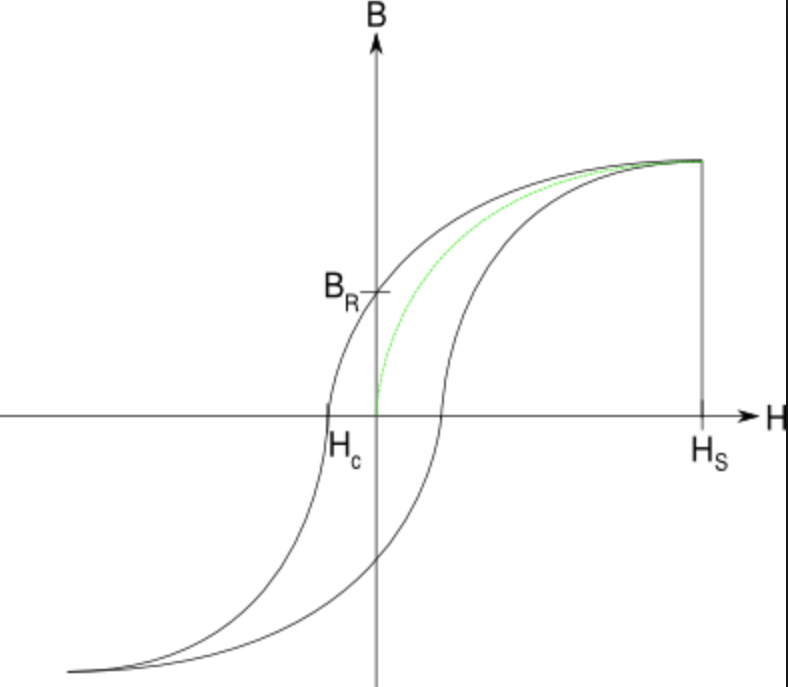
\includegraphics[max width=0.7\linewidth]{/tex/2iteration/billeder/Hysteresekurve.png}
	\caption{Hysteresekurve}
	\label{fig: Hysteresekurve}
\end{figure}
\textbf{Tænker teorien her er lidt tynd, eller er det nok??}

\subsection{Design}
Først og fremmest findes ripplestrømmen, som skal løbe i transformatoren. Her er der taget udgangspunkt i, at designe den efter $60\percent$ af udgangsstrømmen. Dette er et tradeoff mellem størrelsen på ripplen og hvor høj en induktans vi får i viklingerne. Større induktans kræver flere vindinger og giver dermed mere tab.
\begin{equation} \label{I_ripple_CCM}
I_{ripple} = 0.6 \cdot \frac{V_{out} \cdot I_{out}}{V_{inmaks} \cdot   D_{min}} = 2.13A
\end{equation}
Den nødvendige induktans det kræver for at transformatoren kan rampe op til den nødvendige strøm inden for dutycyclen, udregnes på følgende måde:
\begin{equation} \label{L_CCM}
L = \frac{V_{inmin} \cdot D_{min}}{I_{ripple} \cdot f_s} = 69.43\micro H
\end{equation}
Som beskrevet tidligere skal kernen kunne opbevare den energi som kommer fra primær viklingen, når transistoren er on, for at undgå mætning. Mængden af energi i primærviklingen udregnes ved:
\begin{equation} \label{Primary_energy}
w = \frac{1} {2} \cdot L \cdot {I_{pk}}^2 = 1.083\milli J
\end{equation}
For at beregne den tilladelige mængde energi i transformatoren, skal kernen og kernematerialet kendes. Valget er her faldet på en RM8 kerne og materialet 3f3. RM8 kernens mål gør, at den lige akkurat kan være på printet højdemæssigt. Derudover har Terma tidligere brugt RM8 kerner med 3f3 og har nogle mere præcise mål på AL og air gaps, end der er på datasheets’ne. (Kræver det flere argumenter?)


\noindent Den effektive volumen Ve aflæses for RM8. På databladet for 3f3 aflæses et maks peak af B-feltet til omkring $250\milli T$. Hvis der designes efter, at transformatoren vil operere med et højere B-felt, vil man altså risikere at kernen går i mætning. Yderligere findes permeabiliteten for 3f3 materialet uden luftgap. Med disse oplysninger vil transformatoren kunne opbevare følgende energi:
\begin{equation} \label{Energy_no_gap}
w_{kerne} = \frac{1} {2} \cdot \frac{1}{\micro_e} \cdot B^2 \cdot V_e = 53\pico J
\end{equation}
Det er tydeligt at den nødvendige energi på ingen måde kan opbevares i kernen. Da ferrit kan opbevare så lidt energi som det er tilfældet, kan det estimeres at al energien vil blive opbevaret i det luftgap, der designes. Derfor kan permeabiliteten ses som $\micro_0$ i den nye beregning. Den effektive volumen deles op i luftgap og $Al$, så luftgapet kan isoleres. Med dette kan luftgapet beregnes: 
\begin{equation} \label{Airgap}
l_g = \frac{L \cdot {I_{pk}}^2 \cdot \micro_0}{B^2 \cdot A_0} = 690.98\micro m
\end{equation}
Med den ripplestrøm der i første omgang er benyttet, skal der bruges et air gap på ca. $691\micro m$. Den nærmeste air gaps værdi for 3f3 ligger på $488\micro m$ hvilket giver en Al på $160\nano H$. (Dette er ikke databladets værdi, men en værdi der er blevet givet fra Terma, som har testet databladets værdier til ikke at være korrekte.) Det vil ikke fungere, derfor udregnes en induktans, der passer til det air gap i stedet: 
\begin{equation} \label{L1}
L_1 = \frac{l_g \cdot B^2 \cdot A_0}{{I_{pk}}^2 \cdot \micro_0} = 49.035\micro H
\end{equation}
Med kendt Al og induktans kan vindingstallet beregnes. Da der i 2. iteration bruges en 1:1 transformator er dette både for primær og sekundær vikling:
\begin{equation} \label{N}
N = \sqrt{\frac{L_1}{A_L}} = 17.5 \approx 18
\end{equation}
Det passer fint med 18 viklinger på hver side, hvor induktansen igen bliver lidt anderledes når vindingstallet rundes op. 
\begin{equation} \label{L1}
L_2 = N^2 \cdot A_L = 57.76 \micro H
\end{equation}
Med fastlagt induktans kan ny ripple- og peak strøm beregnes.
\begin{equation} \label{I_ripple_CCM}
I_{ripple} = \frac{V_{inmin} \cdot D_{max}}{L_2*f_s} = 2.24A
\end{equation}
\begin{equation} \label{I_pk_CCM}
I_{pk} = \frac{V_{out} \cdot I_{out}}{V_{inmin} \cdot D_{maks}} + \frac{I_{ripple}}{2} = 5.64A
\end{equation}

\subsection{Simulering}
I Pspice er kernen og materialet afprøvet, hvor resten af kredsløbet har været med ideele komponenter, for at kontrollere strømme og B-H kurve. Her ses den pspice-model af kernematerialet som bruges:
\begin{figure}[H]
	\center
	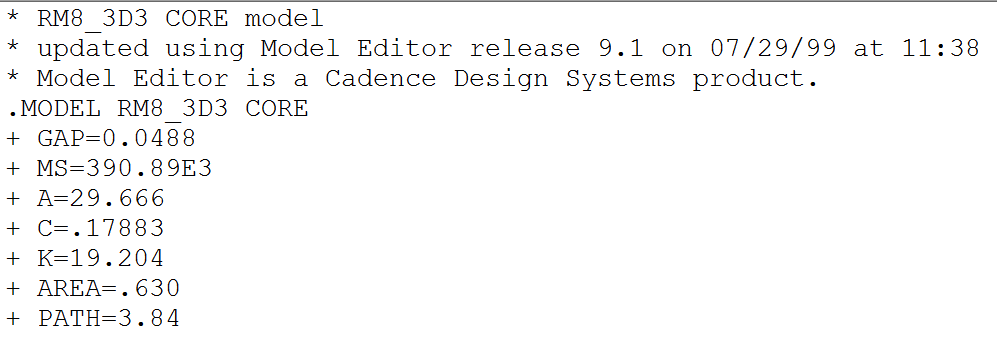
\includegraphics[max width=0.7\linewidth]{/tex/2iteration/billeder/Kernemodel.png}
	\caption{Kernemodel for RM8 3f3}
	\label{fig: Kernemodel}
\end{figure}
Kernemodellen for en 3f3 kerne er indsat, hvor det udregnede air gap også er indtastet. Derudover er der 19 vindinger på primær og sekundærspole. Ellers ingen ændringer i forhold til den rent ideele simulering. Først ses simuleringen af strømmene i transformatoren på primær og sekundær side.
\begin{figure}[H]
	\center
	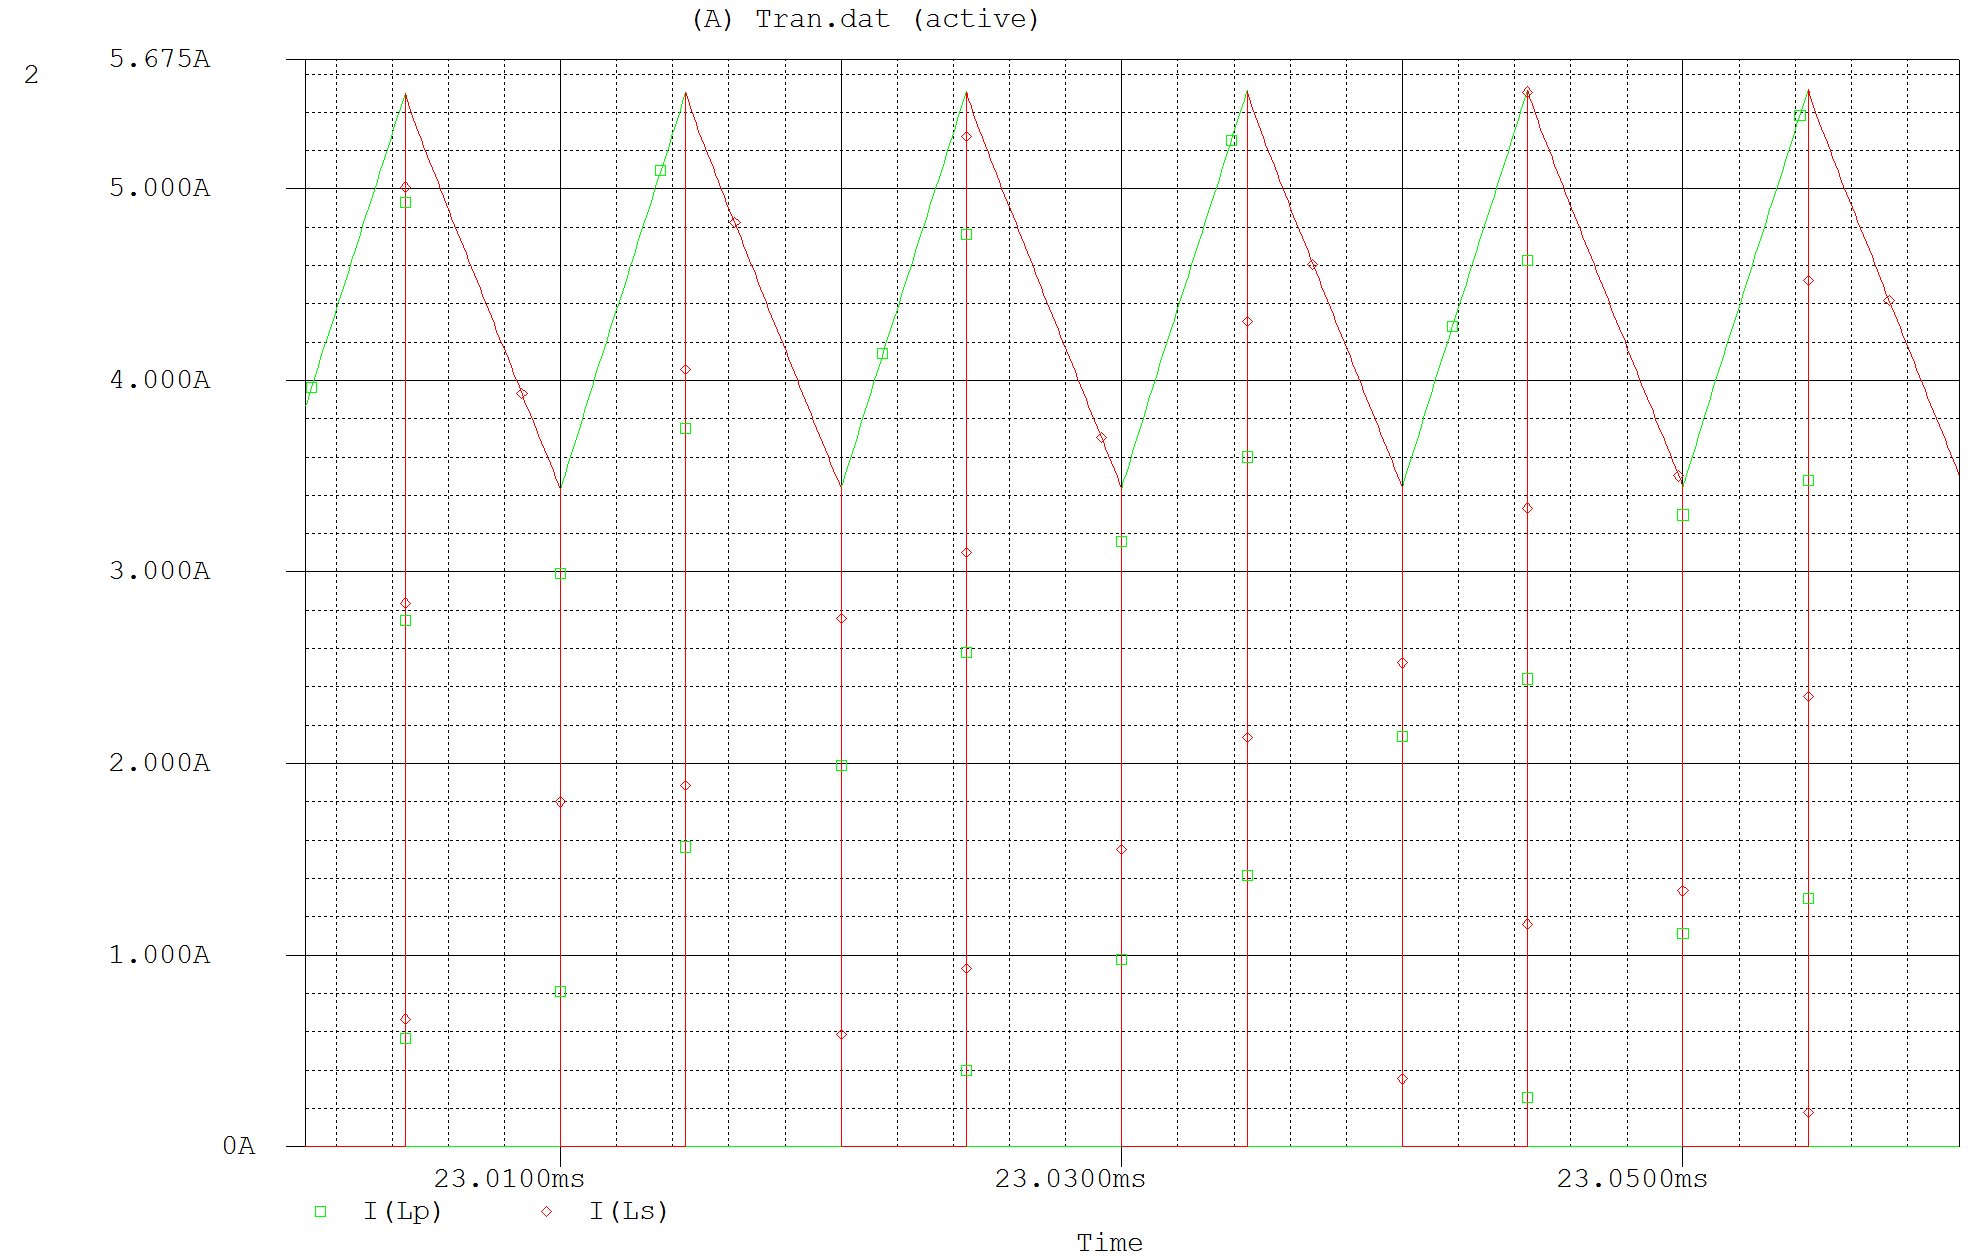
\includegraphics[max width=0.7\linewidth]{/tex/2iteration/billeder/Strom_pri_sek.png}
	\caption{Strøm i primær- og sekundærvikling}
	\label{fig: prisek_strom}
\end{figure}
Det ses tydeligt, at der som ventes køres i CCM, da ripplestrømmene ikke når ned til 0. Ripple- og peak strøm er, som det ses, ens for primær og sekundær, og aflæses til hhv. $2.27A$ og $5.69A$. Det passer fint med det udregnede på $2.24A$ og $5.64A$.
På figur~\ref{fig: RMS_trans} ses RMS strømmene:
\begin{figure}[H]
	\center
	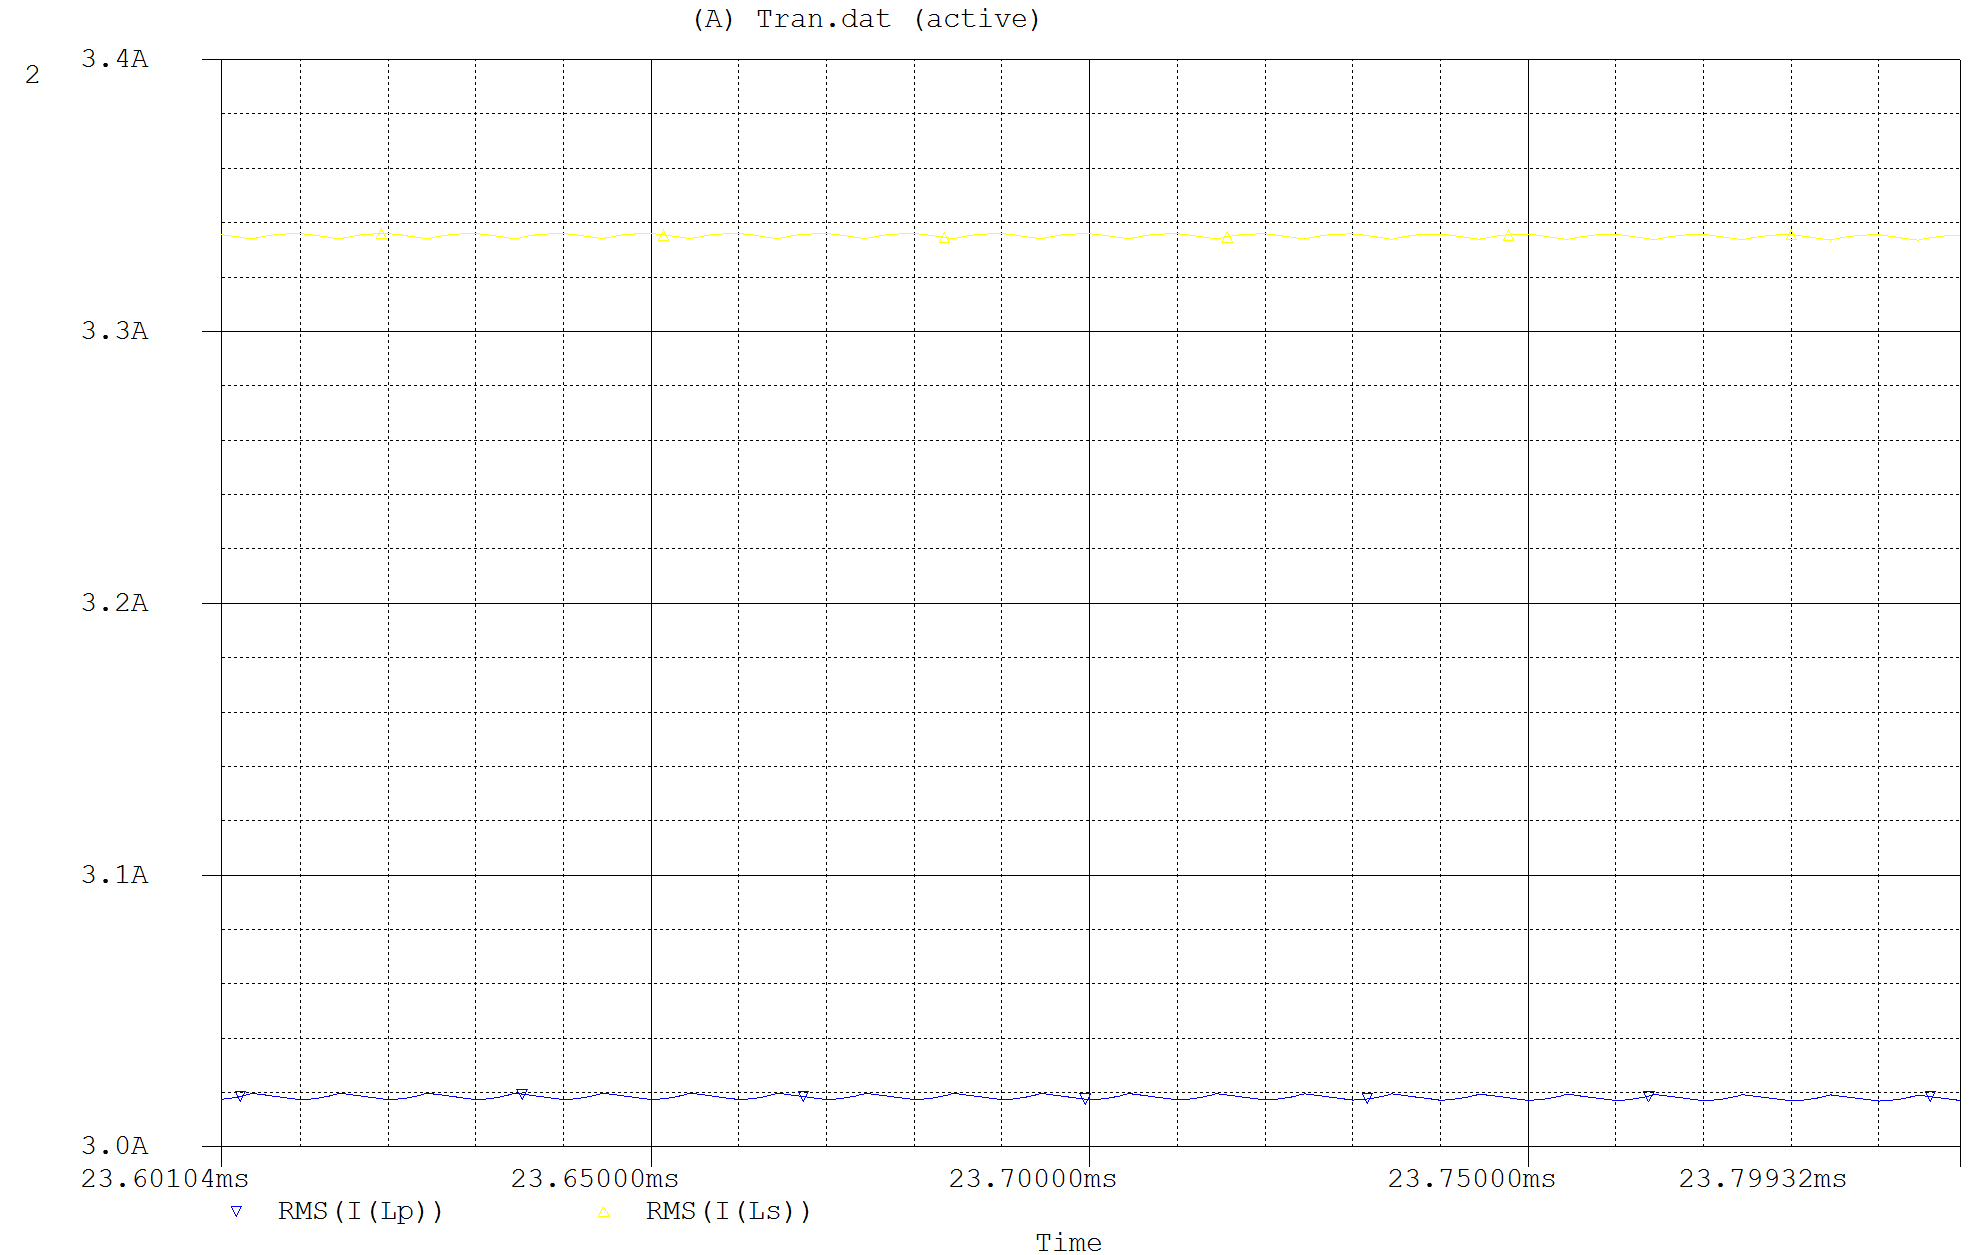
\includegraphics[max width=0.7\linewidth]{/tex/2iteration/billeder/RMS_transformator.png}
	\caption{RMS strømme i transformator (blå=primær og gul=sekundær)}
	\label{fig: RMS_trans}
\end{figure}
Her aflæses den primære til $3.01A$ og den sekundære til $3.33A$, hvilket igen stemmer godt overens med det beregnede på $3.02A$ og $3.36A$.


\noindent Herefter kigges på hysteresekurven, og sikres at den ikke kommer langt over de $250\milli T$, som der er designet efter:
\begin{figure}[H]
	\center
	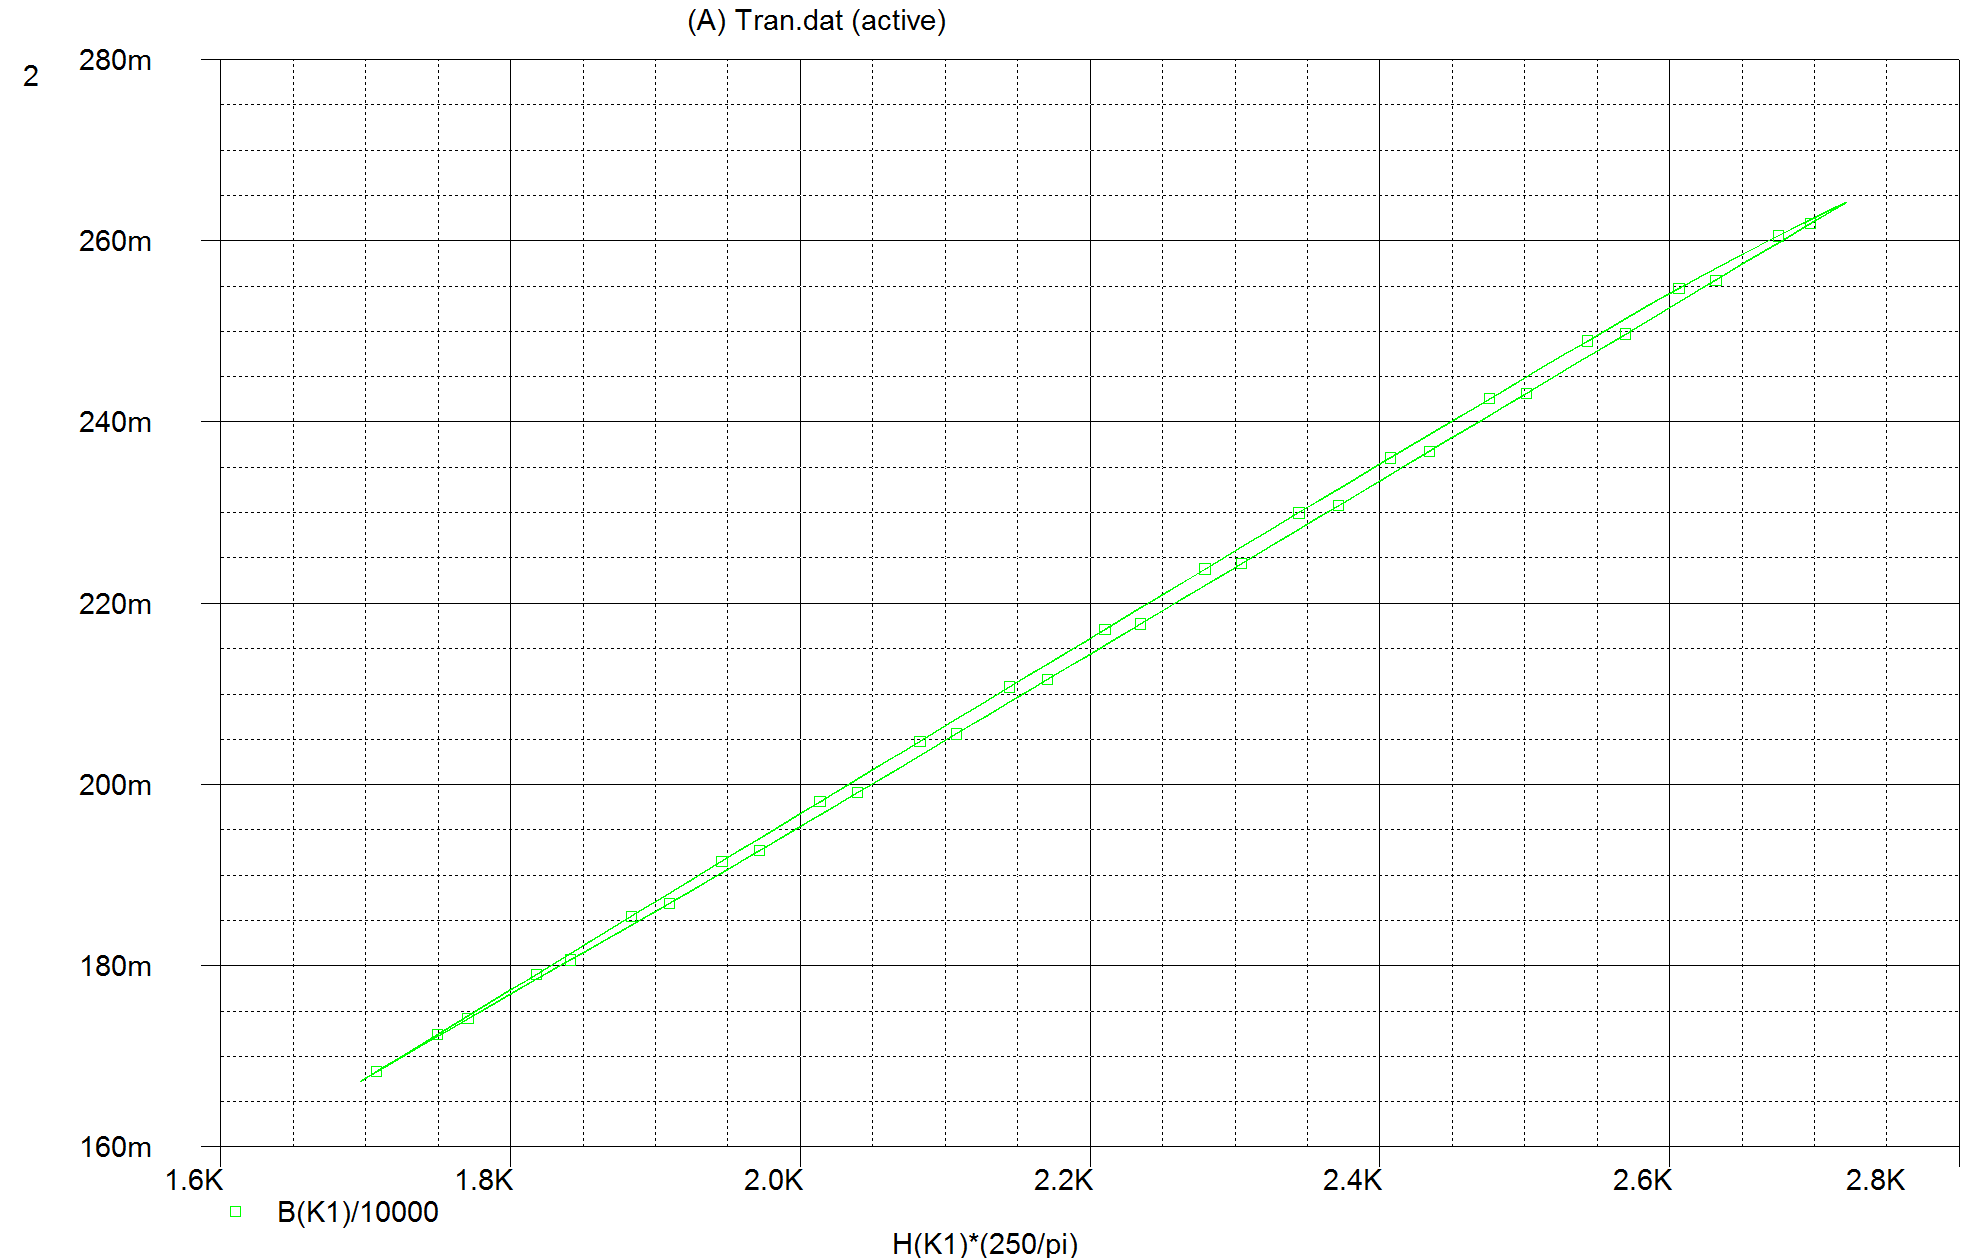
\includegraphics[max width=0.7\linewidth]{/tex/2iteration/billeder/Hysterese_trans.png}
	\caption{Hysteresekurve for transformatoren}
	\label{fig: Hysterese_trans}
\end{figure}
Peak fluxen ligger på ca. $265mT$ hvilket igen passer fint med det der er designet efter. Yderligere ville man kunne se i toppen og bunden af kurven, hvis den gik i mætning, hvilket den ikke gør her.
Tabet i selve kernen er simuleret ved at tage effekten ved den primære vikling i forhold til den sekundære vikling. Tages der i pspice en average af dette fås nedenstående kurve:
\begin{figure}[H]
	\center
	\includegraphics[max width=0.7\linewidth]{/tex/2iteration/billeder/tabkerne.png}
	\caption{Simuleret kernetab i transformator}
	\label{fig: Kernetab}
\end{figure}
Tabet er simuleret til at ligge ved ca. $310\milli W$

\subsection{Vikling af transformator}
Det er vigtigt at prøve at udnytte kernens mål fuldt ud når vindingerne vikles. Med RM8 kernen er der en bredde på $8.6\milli m$ og en højde på $3.475\milli m$. Ved 2. iteration forsøges de mål udnyttet bedst muligt.
Først udregnes den nødvendige diameter af tråden, når der skal ligge 18 vindinger per lag. 
\begin{equation} \label{d_trad}
d_{tråd} = \frac{8.6\milli m}{18} = 0.478\milli m
\end{equation}
Dette er dog den samlede diameter, altså inklusiv isolering. Der benyttes en isolering med grade 2, som giver en diameter på ledningen eksklusiv isolering på $0.425\milli m$.(HENVISNING) Transformeren er 1:1, så både primær og sekundær vikles med 18 vindinger per lag. Et lag af hver giver en højde på $0.956\milli m$. Altså ikke i nærheden af de $3.475\milli m$ i højden. Derfor vikles 2 ekstra viklinger i parallel for både primær- og sekundærsiden og får dermed den tredobbelte højde. Der indsættes tape mellem hver af de parallelle viklinger. Det giver samlet en højde på $2.867\milli m$ plus tape. Det giver i alt 6 lag, 3 for primær og 3 for sekundær. Overblikket over viklingen kan ses på nedenstående tegning:
\begin{figure}[H]
	\center
	\includegraphics[max width=0.7\linewidth]{/tex/2iteration/billeder/viklingsoverblik.png}
	\caption{Overblik over viklingsantal og tykkelse}
	\label{fig: viklingsoverblik}
\end{figure}
\noindent Tegnes bunden af transformatoren fås der et overblik over, hvordan viklingerne vikles. Det ses, at primær begynder og slutter i samme sidde af transformatoren, mens sekundær vikles fra den anden side.  
\begin{figure}[H]
	\center
	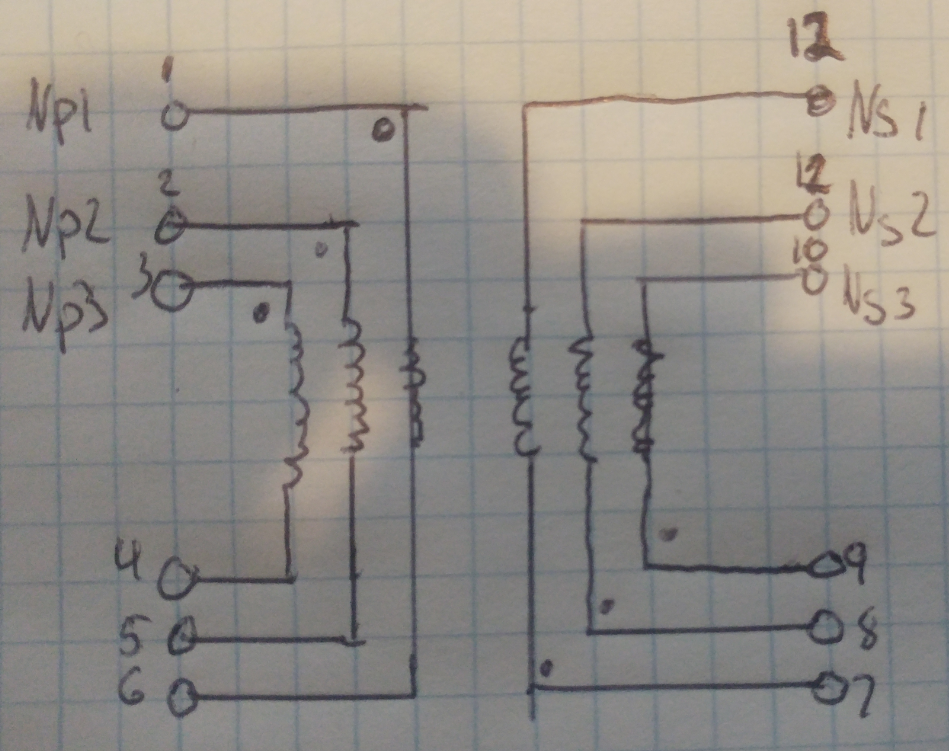
\includegraphics[max width=0.7\linewidth]{/tex/2iteration/billeder/Viklingsbegyndelse.png}
	\caption{Overblik over hvordan viklingerne vikles}
	\label{fig: viklingsbegyndelse}
\end{figure}
\noindent Sidste billede viser hvilken retning der vikles. Her vil primær og sekundær vikles modsatte vej af hinanden, for at få den modsatte polaritet som ønsket.
\begin{figure}[H]
	\center
	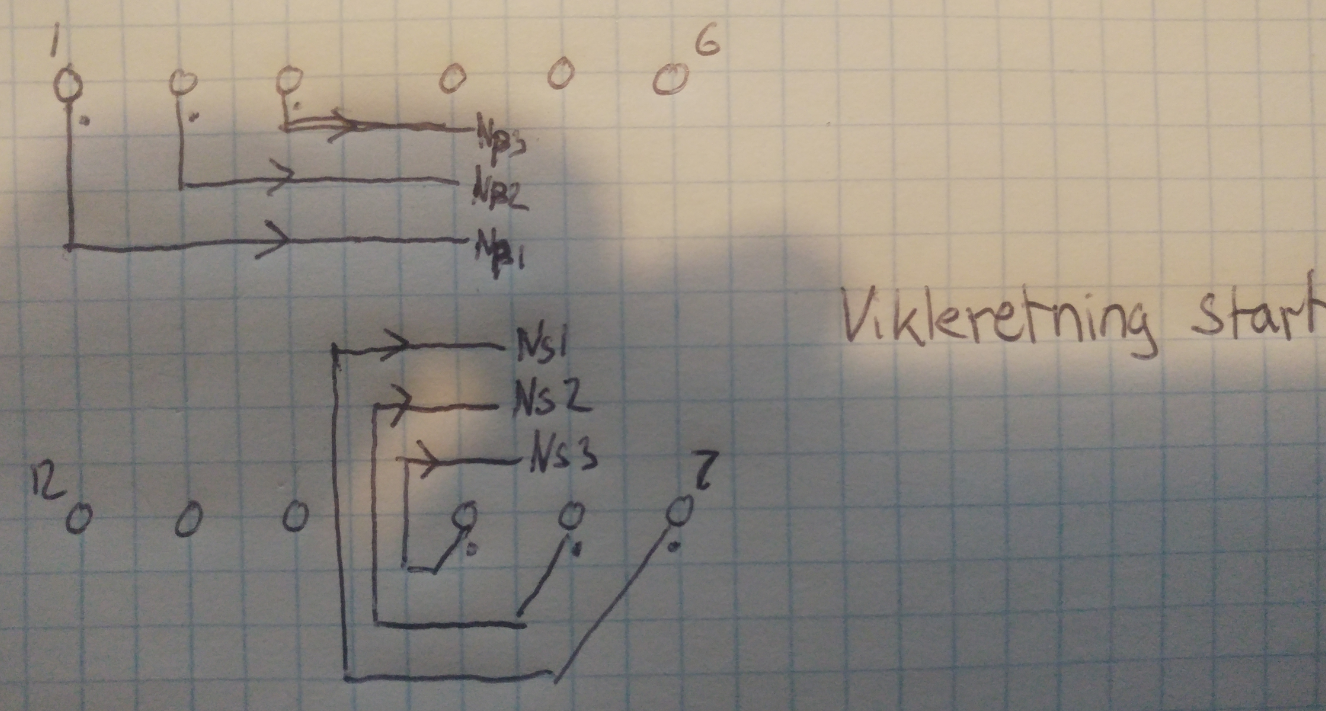
\includegraphics[max width=0.7\linewidth]{/tex/2iteration/billeder/Viklingsretning.png}
	\caption{Begyndelses retning for primær og sekundær}
	\label{fig: viklingsretning}
\end{figure}

\subsection{Realisering}
Mangler billede af transformator. 
På fig ses den viklede transformator. Ved viklingen måtte det erkendes, at der ikke kunne presses 18 vindinger ind, med en ledningstykkelse på $0.425\milli m$, som ellers i forvejen var mindre end den udregnede tykkelse på $0.478\milli m$. I stedet benyttes en tykkelse på $0.425\milli m$ og der tilføjes en ekstra vikling, så det totale antal vindinger ender på 19 per vikling. (ER VI SIKRE PÅ DET IKKE NETOP ER DEN TRÅD VI HAR FÅET?? At trådtykkelsen der står er uden isolering?)

\noindent \textbf{Endelig induktans}


\noindent Da vindingstallet blev 19 i stedet for de 18, er induktansen lidt højere end beregnet i første omgang. Den endelige induktans den viklede transformator beregnes til:
\begin{equation} \label{L_2}
L_2 = N^2 \cdot A_L = 57.76\micro H
\end{equation}
Det ændrer igen en smule på ripple- og peak strømmen i transformatoren:
\begin{equation} \label{I_ripple_final}
I_{ripple} = \frac{V_{inmin} \cdot D_{max}}{L_2*f_s} = 2.01A
\end{equation}
\begin{equation} \label{I_pk_final}
I_{pk} = \frac{V_{out} \cdot I_{out}}{V_{inmin} \cdot D_{maks}} + \frac{I_{ripple}}{2} = 5.53A
\end{equation}

\subsection{Test af transformator}
Transformatoren er testet ved at måle både selvinduktionen i primær- og sekundærviklingerne samt spredningsselvinduktionen. Til dette blev en impedansmåler brugt. 


\noindent Til sådan en måling er det vigtigt, at gøre ledningerne så korte som muligt, da der vil skabes yderligere induktans i dem. Derfor ses på opstillingen på figur… de meget korte ledninger samt der bliver brugt en 4-wire teknik. Det vil sige to ledninger på hver side af det der måles på. Strømmen løber i den ene af ledningerne og??????

\noindent Måleresultaterne tages ved USB ud af impedansmåleren og indsættes i et Excel ark.  

\noindent Først blev en kalibreringsmåling lavet, hvor ledningerne alle målte samme sted. Offsettet herfra er i Excel trukket fra de efterfølgende målinger    

\noindent Herefter måles der på de 2 sider af primærviklingen, mens sekundærsiden holdes åben. På denne måde fås induktansen i den primære vikling. Da transformatoren er 1:1 er det også induktansen i den sekundære vikling. 
\begin{figure}[H]
	\center
	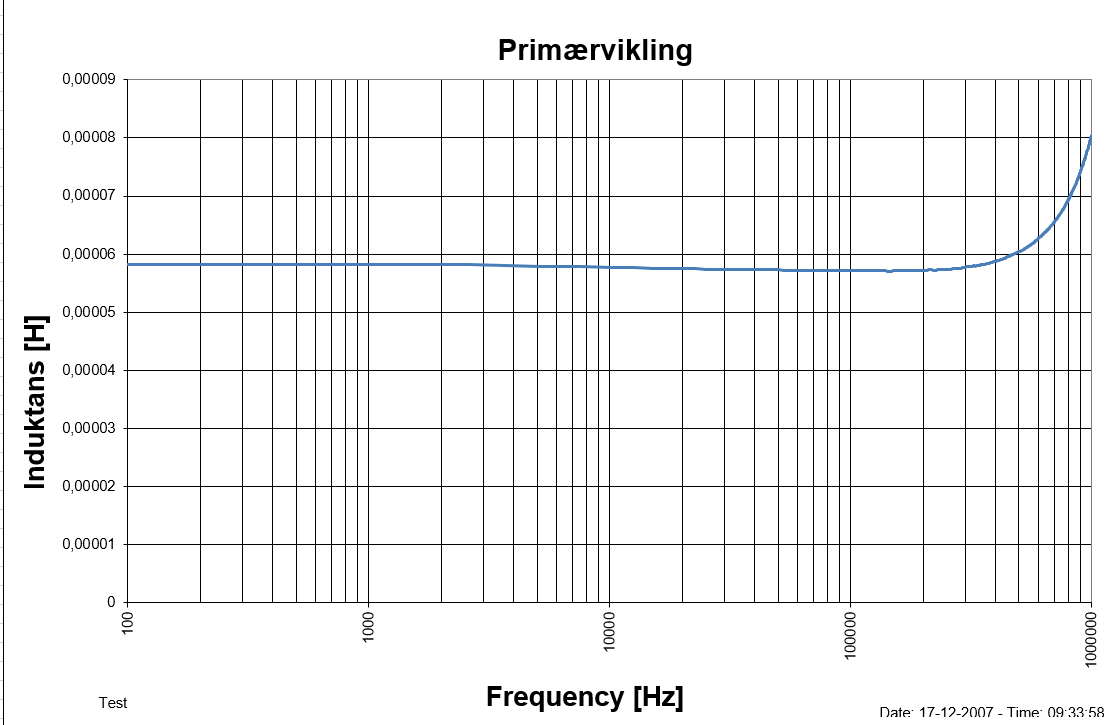
\includegraphics[max width=0.7\linewidth]{/tex/2iteration/billeder/Primarinduktans.png}
	\caption{Målt induktans i primær vikling}
	\label{fig: Primarinduktans}
\end{figure}
\noindent Her er målingen plottet med et frekvenssweep fra $100Hz$ til $1\mega Hz$. Ved de meget høje frekvenser ses det, at kapacitive parasitter tager over. Den skal benyttes omkring 100kHz og her fås værdien i Excel til $57.7\micro H$, hvilket er præcis den induktans der skulle opnås. De præcise målinger kan ses i Excel dokumentet ”Inductance primærvikling” i bilagsmappen. 
Spredningsselvinduktionen fås ved, at kortslutte den sekundære vikling, mens der igen måles hen over den primære vikling. I en ideel transformator bør der her måles 0. Derfor vil induktansen målt her, svare til spredningsselvinduktionen. På samme måde som før er måleresultaterne sendt til Excel hvorudfra en graf kan tegnes. De præcise målinger kan ses i Excel dokumentet ”Spredningsselvinduktion” i bilagsmappen:
\begin{figure}[H]
	\center
	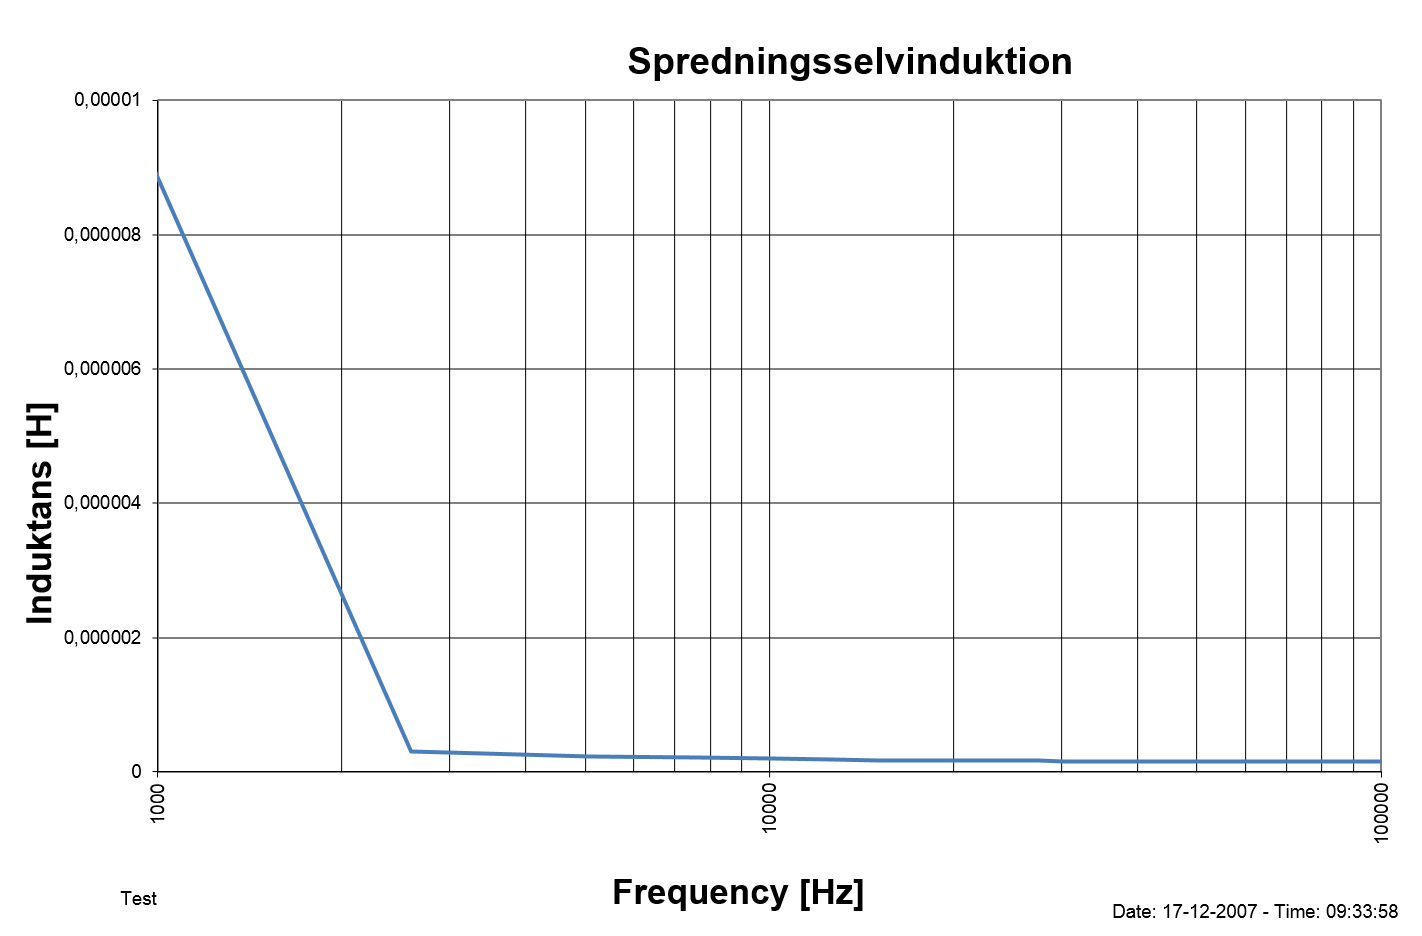
\includegraphics[max width=0.7\linewidth]{/tex/2iteration/billeder/Spredningsselvinduktion.png}
	\caption{Målt spredningsselvinduktion i transformator}
	\label{fig: leakageinductance}
\end{figure}
\noindent Denne graf er fået ud fra et frekvenssweep fra 1kHz til $100\kilo Hz$. Ved de $100\kilo Hz$ er spredningsselvinduktionen på $152\nano H$, hvilket er den værdi der bruges. 

\section{Tab}

\subsection{Kernetab}
Selve kernetabet afhænger af kernematerialet, induktans og strømmen der løber i viklingerne. Først udregnes delta B.
\begin{equation} \label{DeltaB}
\Delta B = \frac{L \cdot I_{pk21}}{N \cdot A_0} = 263.59\milli T
\end{equation}
For at få peak fluxen divideres med 2. Med den kan tabet i kernen per $\frac{\kilo W}{m^3}$
\begin{equation} \label{B}
B = \frac{\Delta B}{2} = 131.79\milli T
\end{equation}
Med den information kigges i databladet under kurven for power loss som funktion af peak flux density.
\begin{figure}[H]
	\center
	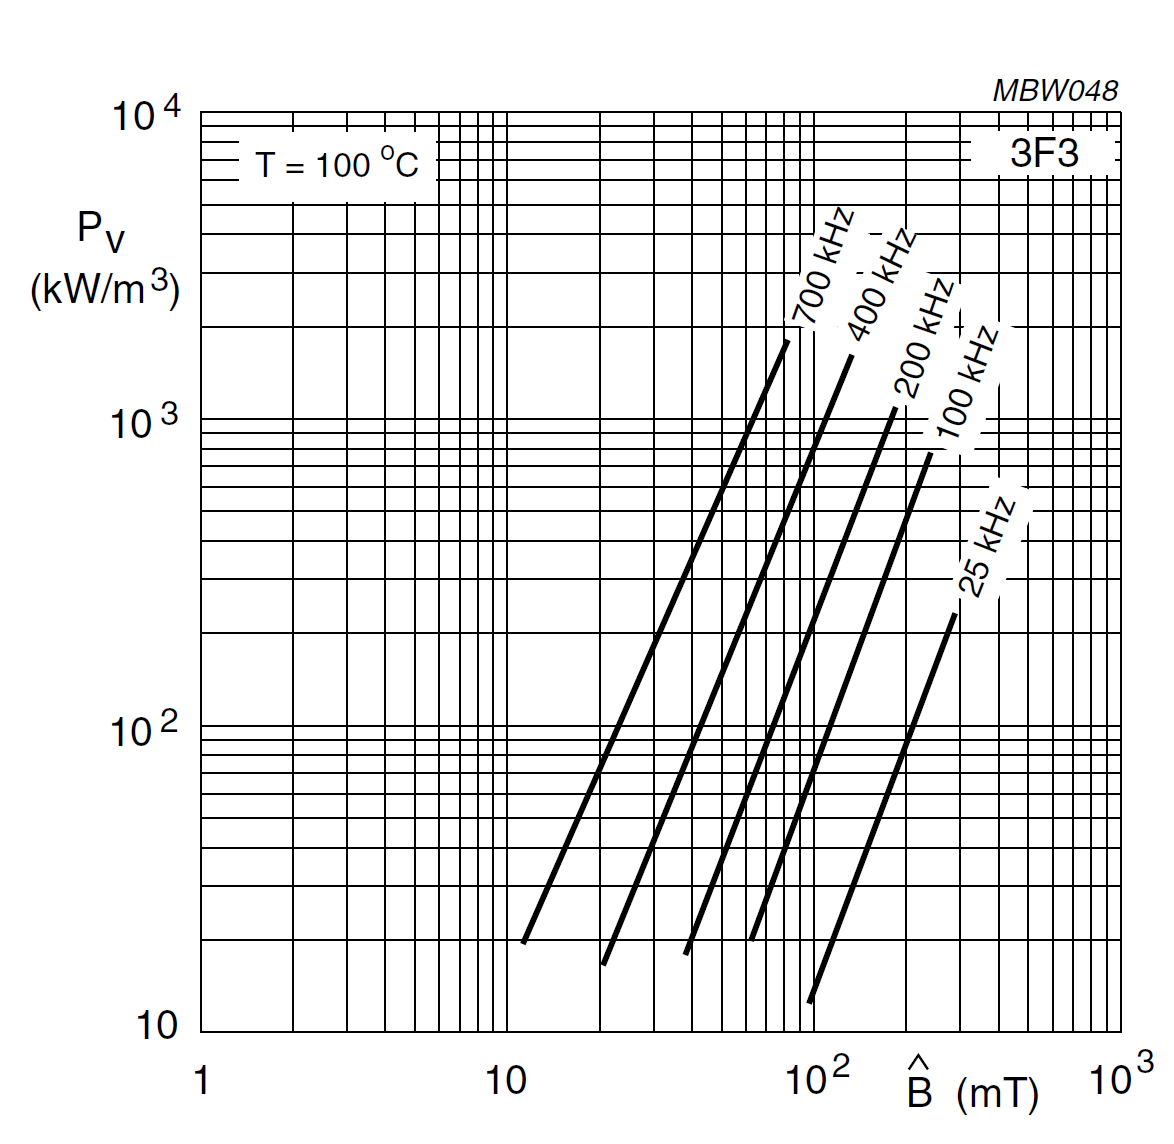
\includegraphics[max width=0.7\linewidth]{/tex/2iteration/billeder/Powerloss.png}
	\caption{Power loss som funktion af peak flux density}
	\label{fig: Powerloss}
\end{figure}
Her ses på de $100\kilo Hz$ ved de ca. $132\milli T$. Det aflæses til et power loss på ca. $150\frac{\kilo W}{m^3}$.
Det samlede kernetab fås med denne værdi ganget med den effektive volumen for RM8 kernen.
\begin{equation} \label{DeltaB}
P = P_V \cdot V_e = 366\milli W
\end{equation}
Dette passer forholdsvis pænt med det simulerede tab i kernen på $310\milli W$.